\documentclass[11pt]{article}
\usepackage{graphicx}
\usepackage{caption}
\usepackage{chngcntr}
\usepackage[section]{placeins} % subsections
\usepackage[round, sort, numbers]{natbib}
\usepackage{makecell}
\usepackage{url}
\counterwithin{figure}{section}
\captionsetup[figure]{slc=off}
\usepackage[left=2cm, right=2cm, top=2cm, bottom=2cm]{geometry} % geometry of page
\setcitestyle{square} % square referencing style
\usepackage[fleqn]{amsmath} % for maths
\usepackage{subfig}
\setlength{\parindent}{0pt} % no indents on new paragraphs
\graphicspath{{Code/Analysis/Figures/}}

\newcommand*\ruleline[1]{\par\noindent\raisebox{.8ex}{\makebox[\linewidth]{\hrulefill\hspace{1ex}\raisebox{-.8ex}{#1}\hspace{1ex}\hrulefill}}}

\usepackage{xcolor}
\definecolor{bookColor}{HTML}{232323}  % 0.90\% of black
\color{bookColor}

\begin{document}
\begin{titlepage}

    \begin{center}
        \vspace*{1cm}
        \Huge
        \textbf{Robotics} \\
        \vspace{0.5cm}
        \LARGE
        \vspace{1.5cm}
        \textbf{G. Sheppard, D. Thomas, J. Doering, J. Matthews, C. Li} \\
        \vfill
        \vspace{0.8cm}
        \Large
        University of Birmingham\\
        Physics and Astronomy Department\\
    \end{center}
\end{titlepage}

\tableofcontents

HERE IS A LIST OF WORDS THAT WE SHOULD CHECK AT THE END TO MAKE SURE WE HAVE ALL USED THE SAME

Double pendulum not triple pendulum \\
Nao not NAO (or other way let's just keep it constant)\\
Posture not position\\
Start-up not startup\\
Large encoder not big encoder (sounds better I think)\\
Rotational not torque\\
Centre point not zero point (as now swings through the centre etc)\\
Set-up not setup (probably this way round who knows tbh)


\section{Abstract}
Wow look at \ref{angleplot}. \cite{Bae2006}.

\section{Introduction}
\subsection{Background}
\subsection{Motivation}
\subsection{Theory}

\section{Connecting To Nao}

\subsection{Nao}
Initial connections to Nao performed using choreograpehn good to familiarise with joint names and connections (graph of joint names, limited by implementation, switched to using the ALProxy and created a joint name model to better understand the joint and connections

Can connect to both virtual and simulated robots in order to check motions before implementing 

Improved on positions from previous years to maximise each posture to extend as far as possible 

Increased the speed of NAOs kicks as previous years limiteted by using the set range of the knee pitch as there max angle as they  assumed this was the largest angle and so the one to maximise

instead based on the range of indidividual positions 

Put in stops to prevent the angle aching to far, same with checking the initial posture when setting up the postures

communicate directly using python scripts


Include diagram of joints and talk about connecting and extracting sensor values and calling joints using python dictionaries:
Normalising speeds, creating algorithms to ensure simultaneity.
Slowing initial speed of NAO to prevent injury during initialisation of positions.
Defining positions to ensure left and right side was symmetric and improved on previous years positions my maximising the range of motion with fail safes to ensure a correct position was reached by comparing joint data with expected position\\

Small amount about compatibility issues and that these were resolved by using the same python SDK and choreagraph versions and running code via linux to prevent issues with compiling and installing: 

Creating 

\subsection{Encoders}
\ruleline{George Sheppard}
There are two sets of hinge encoders used, the large/big encoder, and the small encoders. The large encoder records the angle from the vertical to the largest rod of the swing. The small encoders record the angle with respect to the previous rod, there are 2 on each side of the swing.\\

A large amount of time was invested into connecting to these hinge encoders from any computer other than the lab one. Unfortunately, due to the nature of the shared object files required by the encoders, the set up is complicated and it is advised to use the lab computer when using the hinge encoders.\\

A guide for setting up the hinge encoders is provided in the wiki found in \ref{sec:wiki}.

\subsection{Interface}\label{Interface}
The creation of each individual algorithms required the use of a substantial amount of common code, such as the logic required for: connecting to Nao, collecting values from the hinge encoders and Nao, handling of previous collected values, switching Nao's position, and storage. For this reason an interface was created that functioned as a base that all algorithms were built off, the logic of this base code is illustrated in figure \ref{InterfaceLogic}. The interface starts by collecting all values required for the algorithm decision making process, it then passes these values through the algorithm, depending on the output of the algorithm it will either change Nao's position, switch to the next algorithm, or finish and store the data. It also fixes the sample rate to a specified frequency.\\

    \begin{figure}[!htb]
        \centering
        \captionbox
             {The logic behind the interface, all that required changing was the algorithm logic that the decision making was based on.\label{InterfaceLogic}}
             {\includegraphics[width=1.0\textwidth]{InterfaceLogic.eps}}
    \end{figure}

With this base structure in place, creating an algorithm involved one function that took a set of values, and decided how to react to them, the algorithm had access to all past data to help in decision making. As these algorithms were defined in the same way, it is easy to switch between different algorithms mid swing, such that the motion of NAO could be more stringently controlled. For example NAO could be told to increase to $30^o$, then maintain this amplitude for $10s$, and then finally decrease back down to $0^o$.\\

With this base structure in place, creating an algorithm had two requirements: it took the set of values given to it by the interface, and it returned either 'switch', None, or any of the named positions that were defined in the Robot subsection of the interface e.g. 'Seated', 'Extended' etc.\\

As the interface required the encoders and the robot to connect to, a series of mock classes were created that aimed to replicate their functionality. This meant that away from the lab these fake classes were used as a substitute for the real encoders such that the interface could be developed without errors.

\subsection{Testing}
One of the main advantages of this setup was the ability to test algorithms without connecting to either the robot or the hinge encoders. As all previous data collected in the lab were stored, a setup was developed that read the file in line by line and passed it through the algorithm. This is exactly what would happen in a real test except the real data is replaced with the pre-recorded data.\\
Properties such as the position of Nao at each cycle, and the current algorithm the interface was on is recorded in both the real mode and the testing mode. This meant how each algorithm reacted to different scenarios could be plotted away from the lab, given that pre-recorded data that mimicked that scenario existed.\\
One downside of this method was that the data being fed into the algorithm wasn't reactive to the previous decision of the algorithm, as all the data was pre-recorded. This meant that this method was in no way a full replacement for testing the limits of the algorithm in the lab, but instead was used as a way to check that the algorithm was logically correct before spending limited time with Nao on it.

\subsection{Optimisations}
As discussed in section \ref{Interface}, the interface would record any data relevant to the motion of the swing and Nao. This data could be used to effectively diagnose any problems with the motion, or investigate any other properties of Nao that could be useful in creating new algorithms. This amount of data, however, became a performance issue in certain situations, and this section is dedicated to discussing the optimisations made regarding this.

\subsubsection{Small Encoders}
\ruleline{Jonathan Matthews}
One of the obvious sources of delay in the system is the set of small encoders attached to the swing. These encoders are incredibly useful in modelling the double pendulum of the swing, however, they are irrelevant when the swing is setup in it's simple pendulum mode with all the joints fixed. For these reason there were two setups created for the interface, one that recorded from both the large and small encoders, and one that only recorded from the large encoder only.\\

A method that was investigated to avoid this problem was the introduction of multiprocessing into the interface....
TODO: JONATHAN FINISH THIS BIT, WHY DOESN'T IT WORK, WHAT IS THE SAMPLE RATE OF THE SMALL ENCODERS

\subsubsection{Nao}
\ruleline{George Sheppard}
A second source of delay was the transmission of data to and from Nao, a small subset of this data was paramount to the success of the algorithms, such as the commands for changing the joint positions. A large amount, however, were redundant in certain situations. An example of this was the accelerometer values, initially these were included such that algorithms could be created using only values collected from Nao. A large majority of the time, however, these values were not being used in the algorithms or even looked at when investigating problems with Nao etc.\\

For this reason when creating an algorithm the user could input flags that allowed them to define whether they required these values, when they didn't require these values then fake values would be returned such that performance would increase.\\

Once the optimisations to both the small encoders and the calls to Nao, the interface was able to sample at a maximum of around $200Hz$, at this point the large encoder was restricting any further increases. For most algorithms, however, the workload required by the individual algorithm would restrict this sampling rate before this point. 

\section{Swinging}

\subsection{Webots}
\ruleline{James Doering}
\textit{Here I will talk about Webots, and define each position for Nao with pictures and values for his centre of mass. I will also discuss how we can connect to it with NAOQISIM.}

\subsection{Optimising Nao's Kicks}

\subsection{Rotational Method}

\begin{align}
    &\frac{\Delta E}{E} = 1 - e^{\frac{-2\pi}{Q}}\\
    &\text{At maximum angle},\\
    &E = lmg(1-cos(\theta))\\
    &\Delta E = E(\theta_a) - E(\theta_b)\\
    &\theta_a = \theta_b + d\theta\\
    &\frac{d\theta}{dt} = c - \frac{1-e^{\frac{-2\pi}{Q}}}{dt}\frac{\theta_b}{2}, \, \text{for small angles}
\end{align}
David: Say used previous defined positions, different methods for each algorithm (quarter period, integreation of theory team calculation of max angle), results for each, try to fit maximum amplitude peaks to linear to see if proportional to distance rocked or not, how results varied on different parameters such as if he swings before peak, during, or after, limitations to each method.
Calculations of offset parameters to maximise amplitude gain and comparison of each plot

\subsection{Parametric Method}
Jon: Talk about using the two extra positions defined for this motion from david, the idea behind the algorithm, results try to fit to exponential curve to see if it multiplies amplitude by fixed fraction like worksheet showed, any limitations, were two positions just different in vertical centre of mass or did horizontal distance change too

\begin{align}
    &\theta_a = \theta_b (\frac{L_{squat}}{L_{stand}})^{3/2}\\
    &\theta_a = \theta_b + \frac{d\theta}{dt}dt\\
    &\theta_b + \frac{d\theta}{dt}dt = \theta_b (\frac{L_{squat}}{L_{stand}})^{3/2}\\
    &\frac{d\theta}{dt} = \frac{\theta_b}{dt} ((\frac{L_{squat}}{L_{stand}})^{3/2} - 1)\\ 
\end{align}


\subsection{Damping}
\ruleline{James Doering}
I'll put stuff on how each posture changes his damping coefficient.
I'm also going to talk about how the rotational and parametric methods might look with no damping.
There's a part I need to talk about how rotational the parametric method actually is but IDK where to put it.

\ruleline{George Sheppard}
I'll talk about how much of the damping comes from the air resistance and how much comes from the bearing torque friction, then may calculate the maximum theoretical angle Nao should reach


\section{Single Pendulum}
\subsection{Start-up}
\ruleline{James Doering}
There are multiple different ways to begin a swing from rest, the most intuitive being to "kick off" from the ground - due to Nao's short legs, this was not achievable.This was solved in previous attempts by using a weighted box to kick away from, or by manually pushing Nao, giving the initial amplitude required for normal swinging to be effective. In order to achieve our goals of a fully self-sufficient swinger, a dedicated start-up algorithm was developed. The method is simple - Nao kicks into the extended posture, waits a quarter period, kicks into seated, and then loops between waiting a half period and kicking into the next posture. The initial quarter period wait is used to account for Nao beginning in the centre of his swing, not at the edge. \\

As can be seen in figure \ref{fig:startup}, this method is blah blah blah... The period was calculated from previous data of nao swinging blah blah... noteably, the period of the swing changes slightly depending on the posture, but this was not considered in the code due to the difference in timing being miniscule... \\

This script also offers a good comparison for mass vs no mass etc etc etc etc etc etc etc...



\subsection{Timing via Angular Velocity}
\ruleline{George Sheppard}
To create algorithms that are efficient at applying Nao's energy into the motion of the swing requires an accurate estimate of the maximum angle of the swing, or the time at which this occurs. To early a swing dissipates the energy, and too late doesn't take advantage of the boost in velocity caused by changing position.\\
For this reason a discussion of the best method for determining the maximum of the swing is outlined below.

\ruleline{Chenglong Li}
The angular Velocity algorithms uses the fact that the sign of the angular velocity will change just after the Nao hits its maxima. Therefore one can instruct the Nao to change its posture whenever the angular velocity change its sign. This algorithm is very easy to implement and very reliable. However, there are two serious weakness for this algorithm.The first one is that this algorithm do not learn from old data, which means that it will not keep improving itself. Before talking about the second weakness, one should understand the concept of 'offset' for the algorithm. Assuming the algorithm predicts Nao should change its posture at time T or angle A and one would like it to start change its position a little bit earlier before  

\subsection{Timing via Maximum Angle}
\subsection{Timing via Quarter Period}
\ruleline{George Sheppard}
The quarter period algorithm uses the time that the last quarter period of the cycle took to predict the time of the next maximum, and utilizes the fact that Nao's motion only increases in angle by a small amount per cycle. Whenever Nao swings through the centre of the swing, the first thing to calculate is an estimate of the time that Nao actually crossed the boundary. This is important as Nao swings the fastest through the centre, and therefore the first time recorded after he crossed may not be close enough to the true time. Shown in figure \ref{InterpolationDiagram} is a diagram of this situation. 

    \begin{figure}[!htb]
        \centering
        \captionbox
             {Illustration of the values of the swing, before and after the crossing point.\label{InterpolationDiagram}}
             {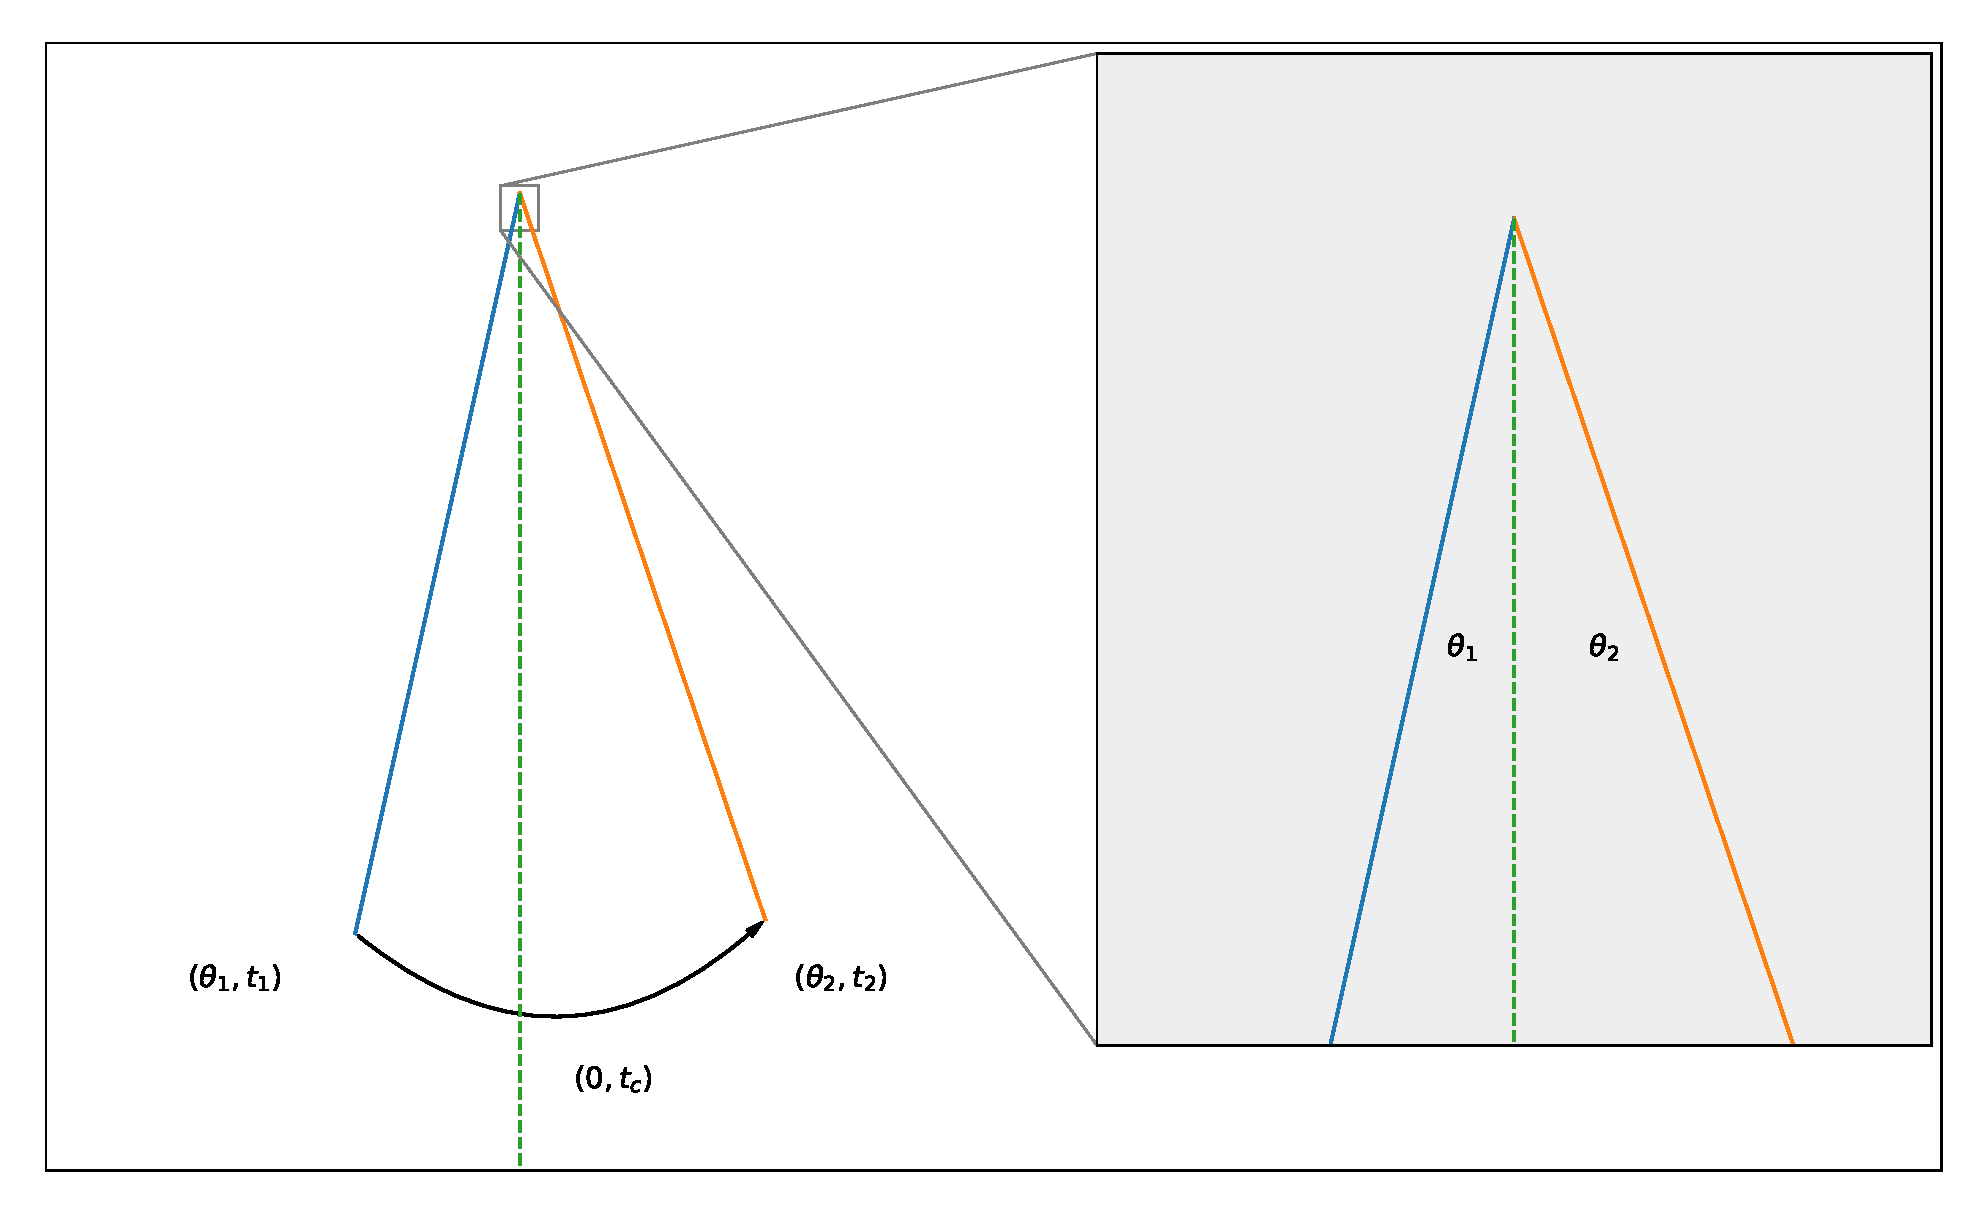
\includegraphics[width=1.0\textwidth]{InterpolationDiagram.eps}}
    \end{figure}

For angle and time $(\theta_1, t_1)$ before the crossing, and $(\theta_2, t_2)$ after the crossing, a linear interpolation can be applied to give a more accurate estimate of the true zero point crossing. This is calculated using

\begin{equation}
    t_c = t_2 - (t_2 - t_1) \frac{|\theta_2|}{|\theta_2 - \theta_1|}.
\end{equation}

As is expected for a higher sampling time this error on the true centre time is smaller. The second value to calculate is the time at which Nao was at the last angle maxima. This can be done simply as all previous values of the encoder are recorded. One small complication is the introduction of local maximas, these occur more often at low amplitude swings due to the jolted motion of Nao's movement, and need to be filtered out to allow a better estimate for the maximum angle time. To filter these local maxima out the moving average of the encoder values is calculated, this smooths the data, figure \ref{MovingAverageDiagram} shows a comparison between the moving average of some example data, for this example the latest local maximum would be the calculated max time, but after using the moving average the estimate is much closer to it's true point. Using the modified encoder values the time of the maximum can be determined, and therefore the quarter period of the swing can be calculated. \\

    \begin{figure}[!htb]
        \centering
        \captionbox
             {Comparison of angle data before and after a moving average is applied.\label{MovingAverageDiagram}}
             {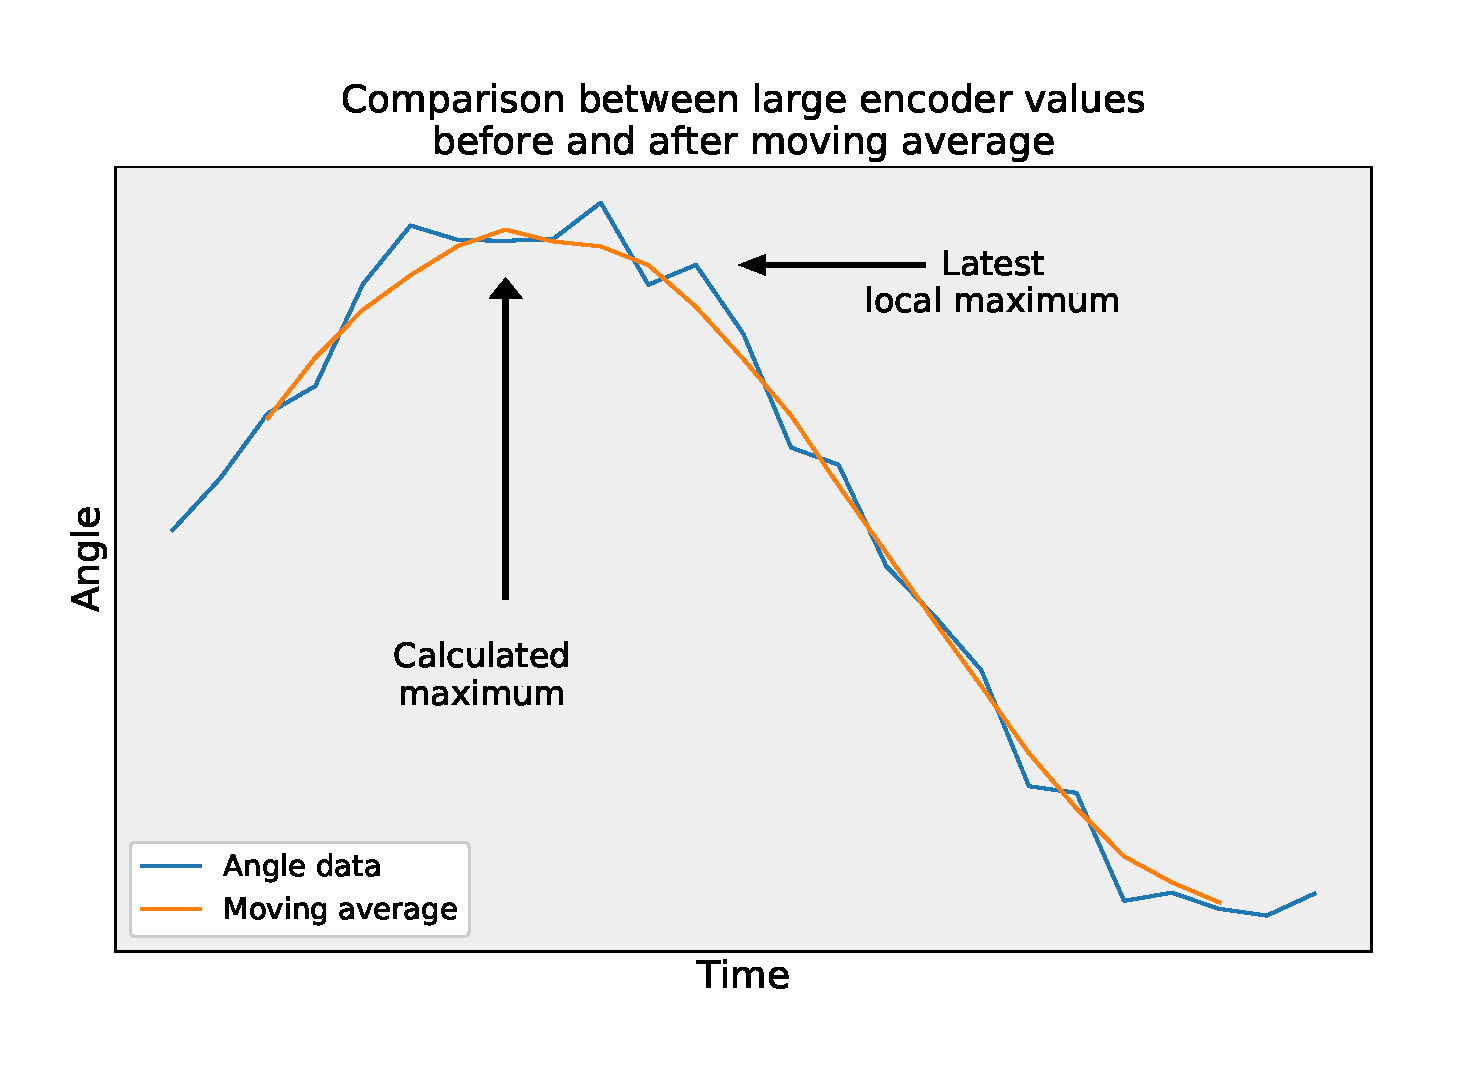
\includegraphics[width=1.0\textwidth]{MovingAverageDiagram.eps}}
    \end{figure}


This process is repeated every half period, whenever Nao crosses the centre point, such that the next maxima time can be calculated before it is reached. From here the only decision that needs to be made is whether it is better to swing before the maxima, at the maxima, or after the maxima for the greatest amplitude swing. An advantage of this algorithm is that the estimate of the period is constantly updated, such that the calculation of the maxima time remains accurate for all amplitudes (as long as there is sufficient build up time to calculate the previous period).


TODO: Advantages and disadvantages of this method
Advantages: Can predict much before the peak allowing offset to decide when is best  
Disadvantages: Only works for small amplitude increases at a time, linear interpolation only works for fast sample speed, smoothing won't remove all local maxima

\subsection{Increasing QP Rotational}\label{Increasing QP Rotational}
\subsection{Increasing QP Parametric}
\subsection{Maintain}
\ruleline{George Sheppard}




\subsection{Decreasing}


\subsection{Dicussion}

\section{Double Pendulum}
\subsection{Start-up}
\ruleline{James Doering}
How is this different to the single pendulum version? Need data on low angle oscillations. How should tactics change?

\subsection{Adjusting Algorithms}
\ruleline{George Sheppard}
To adjust for the new setup of the swing, the single pendulum algorithms needed to be adjusted such that they would account for the motion of the swing below the hinges. For this reason a new coordinate system was defined that took into account the angle of the small encoders. This new coordinate system was defined by an angle named the 'total angle', and a diagram of this angle is shown in figure \ref{} TODO: THIS FIGURE. The large encoder value used previously in all single pendulum algorithms was then replaced with this new total angle to create the new algorithms.

\subsection{Increasing QP Rotational}
From initial experimentation with the double pendulum, it was found that the period of the motion depended largely on the specific motion of the swing below the first now opened hinge. This motion is large when Nao implements the rotational motion seen in section \ref{Increasing QP Rotational}, and as such the angular velocity timing method was decided to be optimum for a rotational motion.\\

The adjusted angular velocity was used to decide when Nao has reached the maximum of his swing, however, there were other adjustments that needed to be made. The first of these adjustments was reducing the speed of Nao's motion. This is because when Nao was switching postures at the maximum speed, the motion of the rods below the first hinge became very chaotic, and ultimately caused a reduction in the total swinging angle. By reducing the posture switching speed to half of the maximum this motion was mostly under control, such that there was mostly a smooth swing.

TODO: RESULTS OF THIS
TODO: PROS AND CONS OF THIS

\subsection{Increasing QP Parametric}



\subsection{Discussion}
\subsection{Maintain}
\subsection{Decreasing}

\section{Future Suggestions}
\ruleline{Code Team}
There are several ideas that given a longer amount of time we would have liked to investigate, the first of which is an algorithm based on accelerometer and gyrometer values only. This would be interesting as it would remove the need for any external inputs such as the hinge encoders, and would allow Nao to be operate any swing without additional setup.


\appendix
\section{Appendix}
\subsection{Wiki} \label{sec:wiki}
\ruleline{George Sheppard}
Throughout this project, there were a large amount of issues found when trying to connect to: Nao, Webots, and the hinge encoders etc. For this reason a wiki was created to document how to set everything up correctly. This wiki is available at: https://github.com/GeorgeSheppard/Robotics. Alongside this wiki is the final code, including how to use it, the report, and any analysis files used to create plots. Feel free to clone this repository and add to it such that there remains a comprehensive guide for each year.

\subsection{Webots}
\ruleline{James Doering}
Webots offers a substantial amount of uses - throughout this project Webots was used to test the interface and algorithms away from the lab, and to find accurate estimates for NAO's centre of mass in different positions. However, Webots did not offer much in useful physical simulations - the simulated swing would often fail, and physics would quickly go out of sync if the target frame-rate was missed momentarily. In order to interface with Webots from the NAOQI python library (supplied by Aldebaran/SoftBanks), the NAOQISIM controller was required - this acted as a 'virtual robot' to translate from Python script written with NAOQI to the NAOQISIM controller in Webots, which controlled the simulated NAO. This proved difficult to achieve, only being possible with certain software configurations. It is highly recommended that this is done on a linux operating system, otherwise there will be errors between 32 and 64 bit versions of python and NAOQI/NAOQISIM. The version of NAOQI required to connect to Webots is different to the version required to connect to the real NAO - as of writing, Webots/NAOQISIM requires NAOQI 2.1.4.13, whereas NAO requires NAOQI 1.14.5. Further explanation can be seen on the wiki decribed in section \ref{sec:wiki}.

\bibliographystyle{ieeetr}
\bibliography{References}
\end{document}